\documentclass[12pt]{beamer}



\setbeamertemplate{headline}{
\begin{beamercolorbox}[wd=\paperwidth]{chcolor}
\end{beamercolorbox}
}

%\usepackage[japanese]{babel}
\usepackage{xeCJK}
 \setCJKmainfont[BoldFont=../fonts/AozoraMincho-bold,AutoFakeSlant=0.15]{../fonts/AozoraMinchoRegular.ttf}
%\setCJKmainfont[BoldFont=NotoSansCJKjp-Bold,AutoFakeSlant=0.15]{Noto Sans CJK JP}


\usepackage[size=a0,orientation=landscape,scale=1.4]{beamerposter}
\geometry{paperwidth=1600mm,paperheight=900mm}
\usepackage{amssymb}
\usepackage{amsmath}
\usepackage{dsfont}
\usepackage{gensymb}


\setbeamerfont{title}{family=\rmfamily}
%\setbeamercolor{title}{fg=red!50!blue!30}
 \setbeamercolor{title}{fg=black}
 \setbeamercolor{frametitle}{fg=black}
%\usepackage{fontspec}
\usefonttheme{professionalfonts} % using non standard fonts for beamer
%\usefonttheme{serif} % default family is serif

\setbeamertemplate{frametitle}{\vspace{1mm}\color{black}\bfseries\large\insertframetitle\par\vskip-6pt\hrulefill\par\normalsize\insertframesubtitle}
\setbeamertemplate{footline}{\qquad\color{black}\bfseries\insertframenumber\vspace{3mm}}
%\setbeamertemplate{footline}{\vspace{5mm}}
\setbeamertemplate{itemize item}{\color{black}\tiny$\blacksquare$}
\addtobeamertemplate{footnote}{}{\vspace{-2ex}}

\newcommand\Fontvi{\fontsize{9}{7.2}\selectfont}

\usepackage{xcolor,graphicx}
\usepackage[outdir=figures/converted_figs/]{epstopdf}
\usepackage{subfig,float}
\usepackage[figurename=Fig.,tablename=Tab.]{caption}% center as possible option
\usepackage{booktabs,array,rotating,tabularx}
%\usepackage{verbatim}       %% Doesnt work with beamer

\usepackage[absolute,overlay]{textpos}
%\usepackage[texcoord,
%grid,gridcolor=red!10,subgridcolor=green!10,gridunit=pt]{eso-pic}
\setbeamerfont{footnote mark}{size=\Tiny}

\usepackage{caption}
\DeclareCaptionLabelSeparator{pipe}{ $|$ }% or $\vert$
\captionsetup{
  format=plain,
  justification=raggedright,
  singlelinecheck=false,
  font=small,
  font={bf,sf}, % This covers labelfont and textfont
  labelsep=pipe,
  figurename=Figure
}


%\captionsetup{font={tiny,onehalfspacing}}    %% messes up the footnotes

\def\eq{equation}

\usepackage{hyperref}
 \hypersetup{
    colorlinks=true,
    linkcolor=black,
    filecolor=magenta,
    urlcolor=red,
    bookmarksnumbered=true,
    citecolor=blue
 }
 \urlstyle{same}

%\usepackage[acronym,nonumberlist]{glossaries}
% \makeglossaries
% \loadglsentries{../glossary}

\usepackage{animate}
\usepackage{tikz}
 \usetikzlibrary{positioning}
 \usetikzlibrary{snakes}
%\usetikzlibrary{shapes.misc}
%\usetikzlibrary{decorations}

\newcommand{\putat}[3]{\begin{picture}(0,0)(0,0)\put(#1,#2){#3}\end{picture}}

\title{\newline\newline\newline \bfseries {Major Advanced Topics  \\ 
 \Tiny  26433101}}
\author[Fred]{\textbf{Ongonwou Fred}}
\institute{
        \textbf{Phd Candidate}\\\textbf{\hspace{2mm}2343003}
}
%\date{April 26, 2023}
\titlegraphic{
% \begin{picture}(-100,0)
%  \put(-240,167){
\includegraphics[scale=.28]{ustm_logo.png}}%\footnote{logo USTM}}
%  \put(50,155){
\includegraphics[scale=1.5]{ed-sfa_logo.jpg}}%\footnote{logo ED-SFA}}
% %\put(-150,190){\makebox(0,0)[]{\includegraphics[width=20mm]{example-image-a}}}
% \end{picture}
}




\begin{document}


\begin{frame}%[t]
\frametitle{\Huge
\begin{center}
\vspace{100pt}

Atomic, Molecular and Optical (AMO) Physics \par\vspace{50pt}
\huge
Controling, tracking and visualizing 
matter through the help of radiation \par\vspace{30pt}
{ \Large
Fred. Ongonwou, Department of Engineering Science, Morishita Laboratory,
The University of Electro-Communications}
\end{center}
}

\framesubtitle{
\begin{center}
\large
\textbf{Atomic, Molecular and Optical (AMO) physics} explores how atoms
and molecules interact with light. Using powerful lasers, we can control
electrons, generate new type of light, and even take pictures 
of matter in motion -- at timescales a billion times faster than a camera flash.
These techniques let us probe the structure and dynamics of molecules, 
understand fundamental quantum processes, and build technologies like
quantum sensors, ultrafast microscopes and new light sources. 
AMO physics is the science behind some of the most precise measurements 
and fastest tools ever made. 
\end{center}
}


\begin{textblock*}{\textwidth}(100pt,750pt)
\Large

\begin{equation}
\mbox{Classical physics (High school)} \hspace{250pt}
E = \frac{1}{2}mv^2 - \frac{e^2}{4\pi\varepsilon_0 x} -e \boldsymbol{E}\cdot 
   \boldsymbol{r} \hspace{100pt} \longrightarrow \hspace{100pt}
i\frac{\partial}{\partial t} \psi(\boldsymbol{r,t}) =
  \Big(-i\hbar\frac{\partial^2}{\partial r^2} - \frac{e^2}{4\pi\varepsilon_0 x}
- e\boldsymbol{E}\cdot\boldsymbol{r}\Big) 
\Psi(\boldsymbol{x},t)
\hspace{250pt}\mbox{Quantum physics (University)}
\end{equation}


%\centering
%%\rotatebox{0}{
% \begin{minipage}{0.5\linewidth}
%  \ \textbf{Basic strong field phenomena} \\
% \begin{figure}[tp]
%  \small 1. Multiphoton Ionization (MPI)
%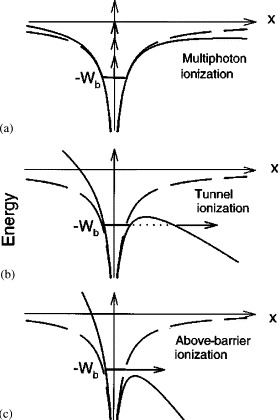
\includegraphics[scale=.9, trim={0 0 0 0},clip]{images/phenomena.png} 
%  \small 2. High harmonic generation (HHG)
%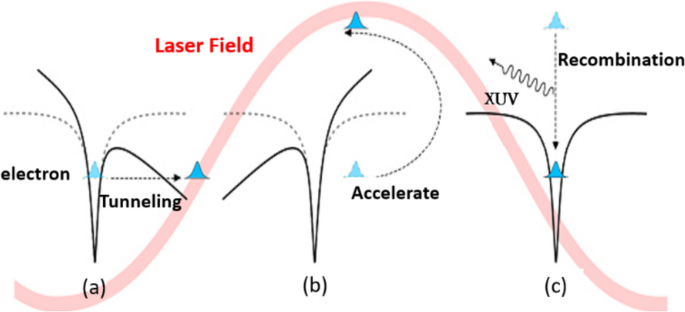
\includegraphics[scale=.7, trim={0 0 0 0},clip]{images/hhg_process.png}
%\vspace{10pt}
% 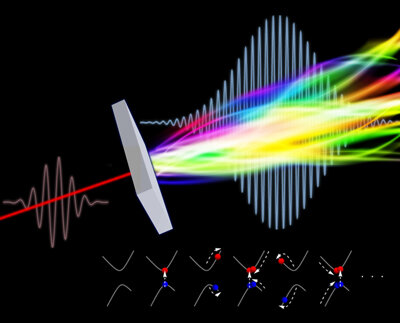
\includegraphics[scale=1., trim={0 80 0 0},clip]{images/modeling-high-harmonic.jpg} 
%  \small 3. Nonsequential double ionization (NSDI)
% 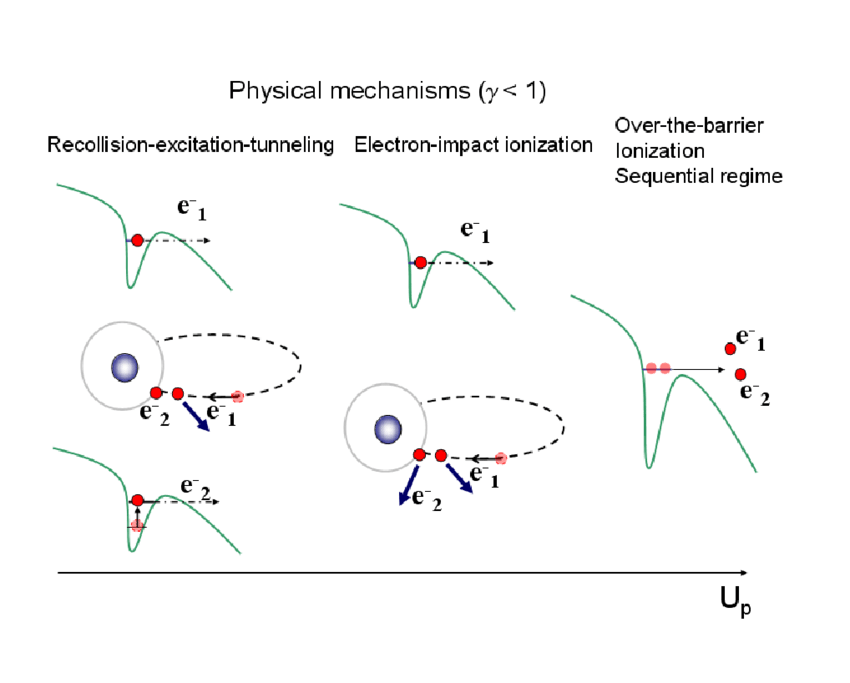
\includegraphics[scale=0.7, trim={0 20 0 0},clip]{images/nsdi_scheme.png}
% 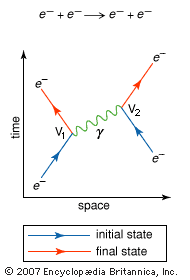
\includegraphics[scale=1.3, trim={0 0 0 10},clip]{images/nsdi_feynman.png}
%%\caption{Eigenvalues.}
%%\label{fig:pemd_0114}
% \end{figure}
%%}
%\end{minipage}
\end{textblock*}

% ----- First column

%\begin{textblock*}{\textwidth}(100pt,1000pt)
%{\huge\textbf {1. Tunnel Ionization}} \\\vspace{30pt}
%%Theory and illustrations to put here
%
%\end{textblock*}

\begin{textblock*}{1000pt}(100pt,1000pt)
%\centering
%\rotatebox{90}{
%  \large \textbf{Have you ever seen a blue laser?}
{\huge\textbf {1. Ionizations}} \\\vspace{30pt}
% \begin{minipage}{0.6\linewidth}
 \begin{figure}[tp]
 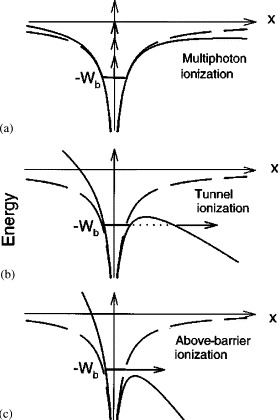
\includegraphics[scale=2., trim={0 0 0 0},clip]{images/phenomena.png} \\\vspace{100pt}
 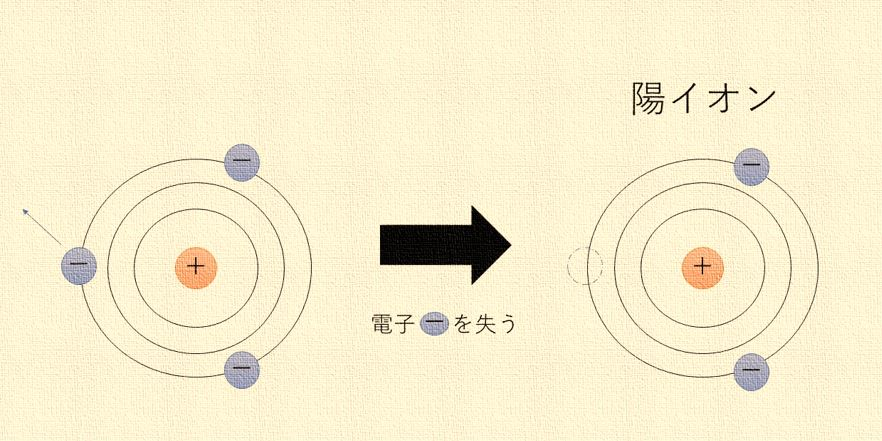
\includegraphics[scale=2., trim={0 0 0 0},clip]{images/ionization.jpg} \\
%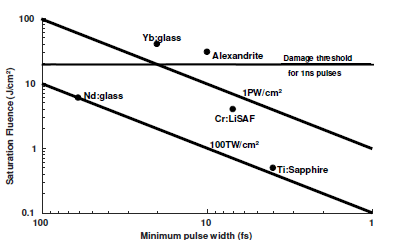
\includegraphics[scale=2., trim={0 0 0 0},clip]{images/intensity_medium.png} \\
%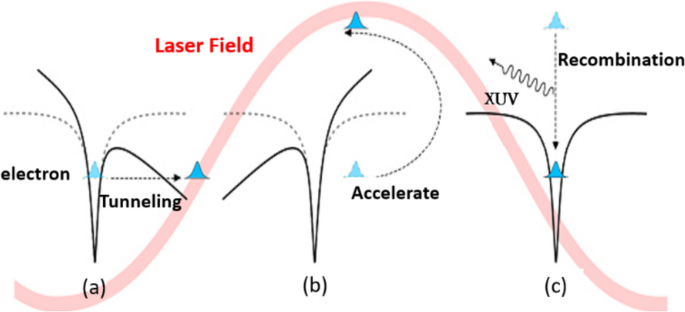
\includegraphics[scale=.50, trim={0 0 0 0},clip]{images/hhg_process.png}

%%\caption{Eigenvalues.}
%\label{fig:pemd_0114}
 \end{figure}

%\end{minipage}
\end{textblock*}



\begin{textblock*}{1000pt}(1200pt,1000pt)
%\centering
%\rotatebox{90}{
%  \large \textbf{Have you ever seen a blue laser?}
{\huge\textbf {2. Multiphoton ionization}} \\\vspace{30pt}
% \begin{minipage}{0.6\linewidth}
 \begin{figure}[tp]
 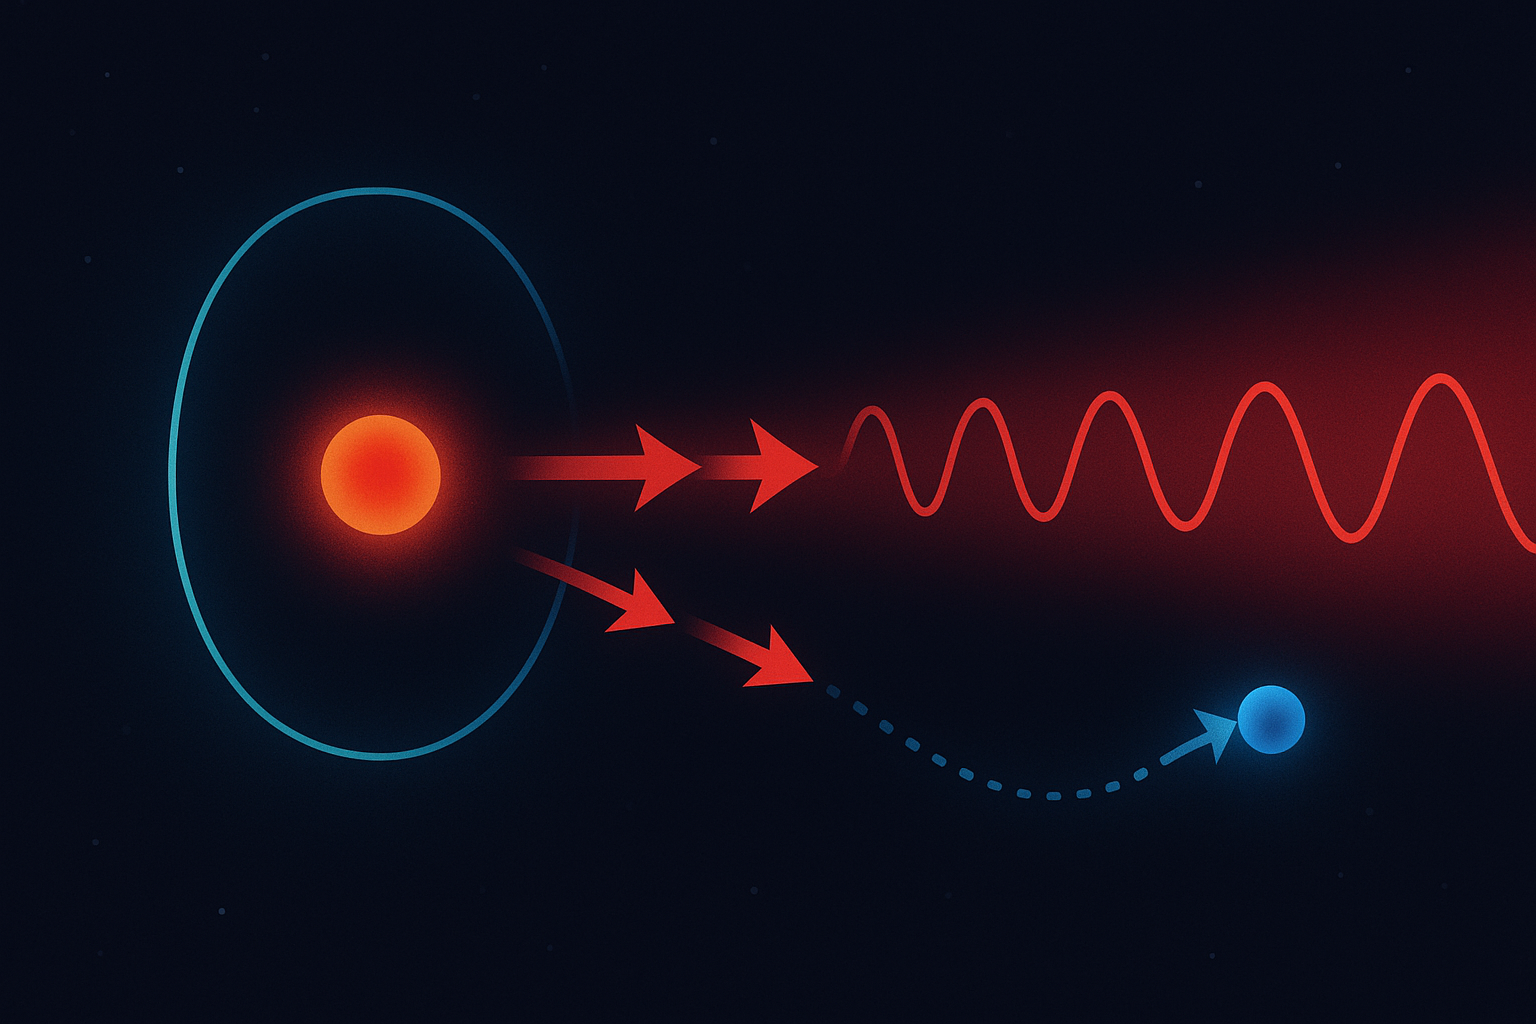
\includegraphics[width=\textwidth, height=400pt, trim={0 0 0 0},clip]{images/multiphoton.png} \\
 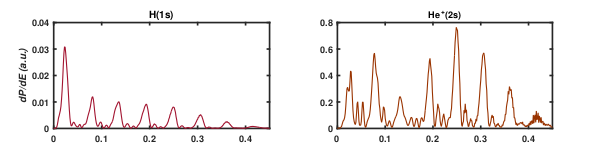
\includegraphics[width=\textwidth, trim={15 10 320 0},clip]{images/ati.png} \\\vspace{20pt}
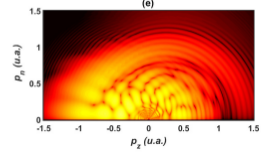
\includegraphics[width=.8\textwidth, trim={30 10 10 10},clip]{images/ati2.png} \\
%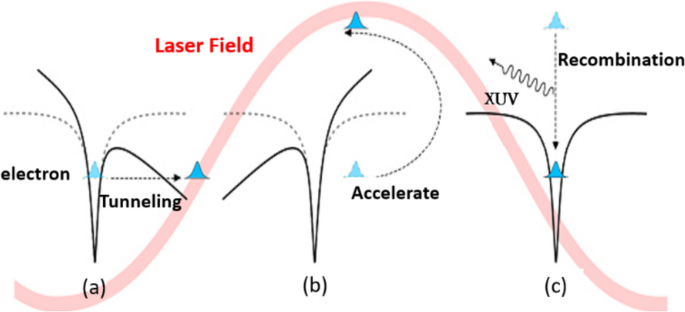
\includegraphics[scale=.50, trim={0 0 0 0},clip]{images/hhg_process.png}

%%\caption{Eigenvalues.}
%\label{fig:pemd_0114}
 \end{figure}

%\end{minipage}
\end{textblock*}


\begin{textblock*}{1000pt}(2300pt,1000pt)
%\centering
%\rotatebox{90}{
%  \large \textbf{Have you ever seen a blue laser?}
{\huge\textbf {3. High Harmonic Generation}} \\\vspace{30pt}
% \begin{minipage}{0.6\linewidth}
 \begin{figure}[tp]
 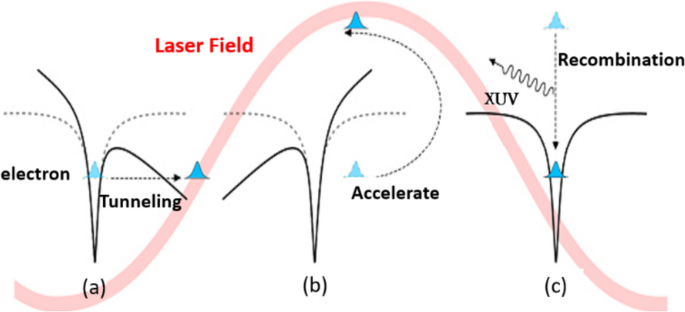
\includegraphics[width=\textwidth, height=300pt, trim={0 0 0 0},clip]{images/hhg_process.png} \\\vspace{50pt}
\textbf{\Large Have you ever seen a blue laser?}
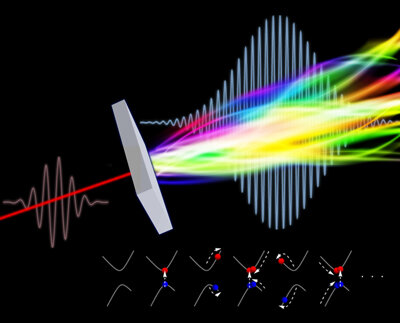
\includegraphics[width=\textwidth,height=300pt, trim={5 90 5 0},clip]{images/modeling-high-harmonic.jpg} \\
 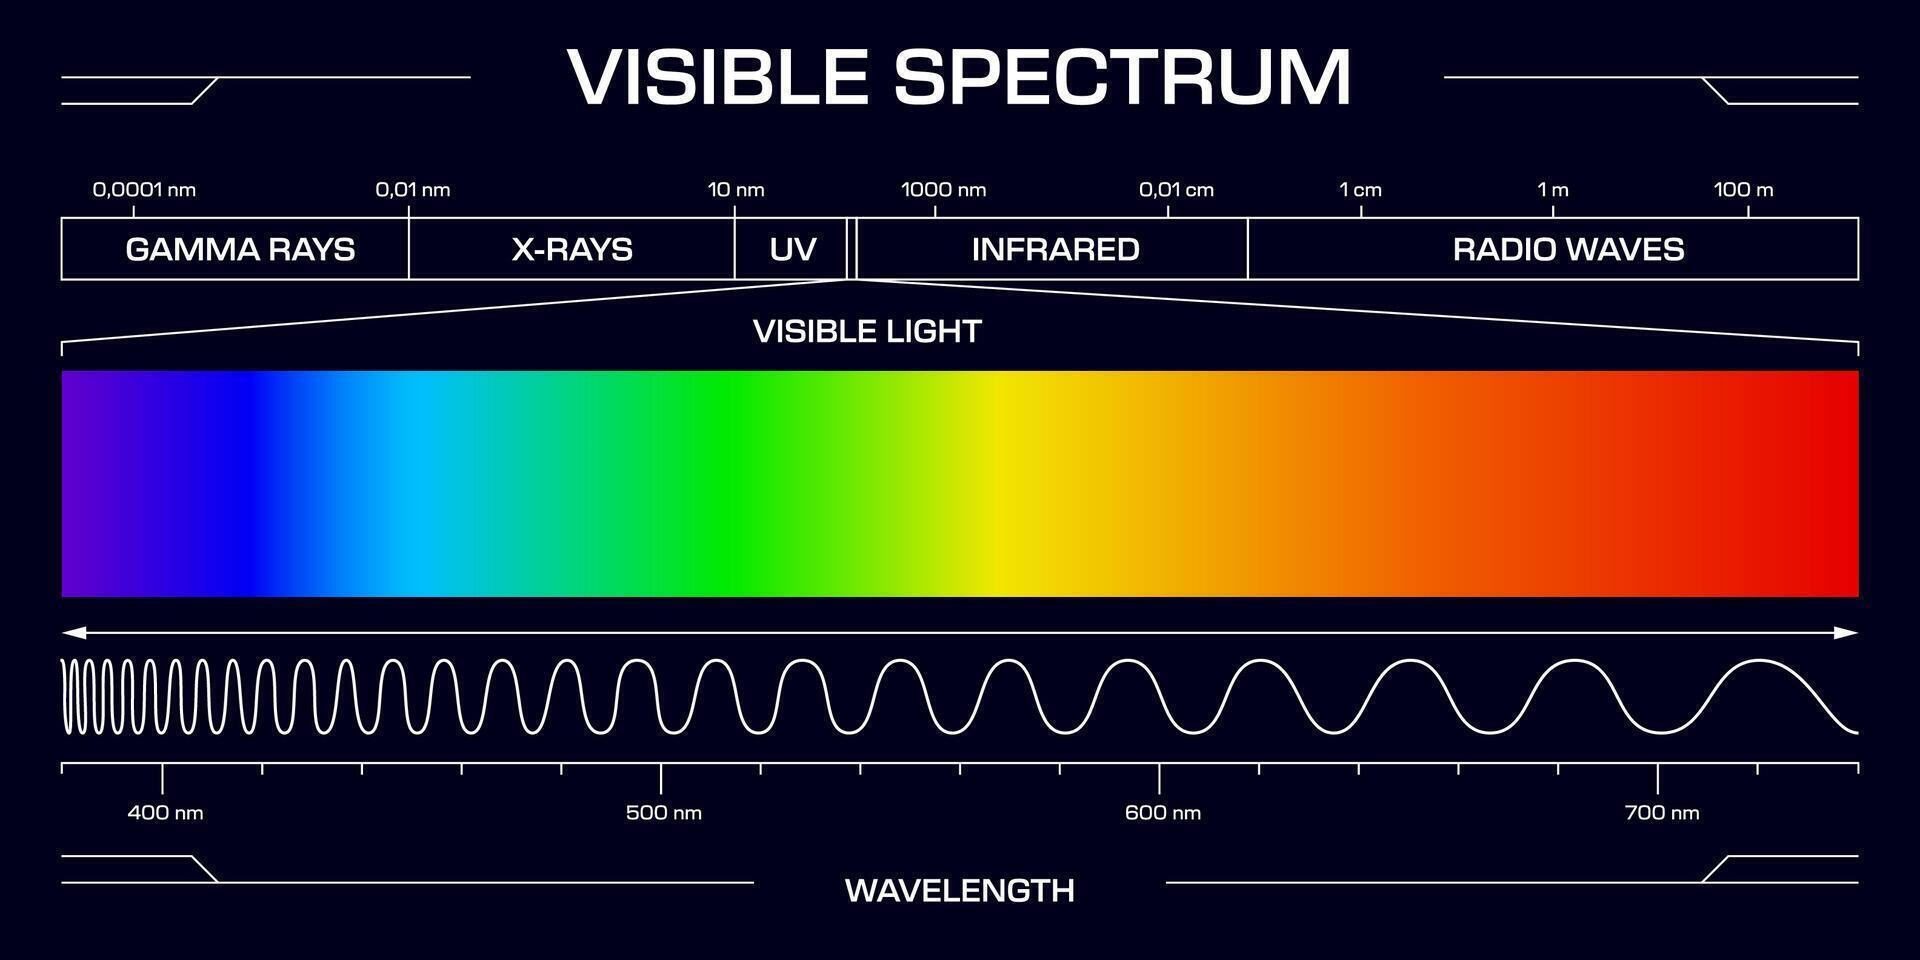
\includegraphics[width=\textwidth,height=300pt, trim={0 0 0 0},clip]{images/visible-spectrum-light-wavelengths-diagram-vector.jpg} \\
 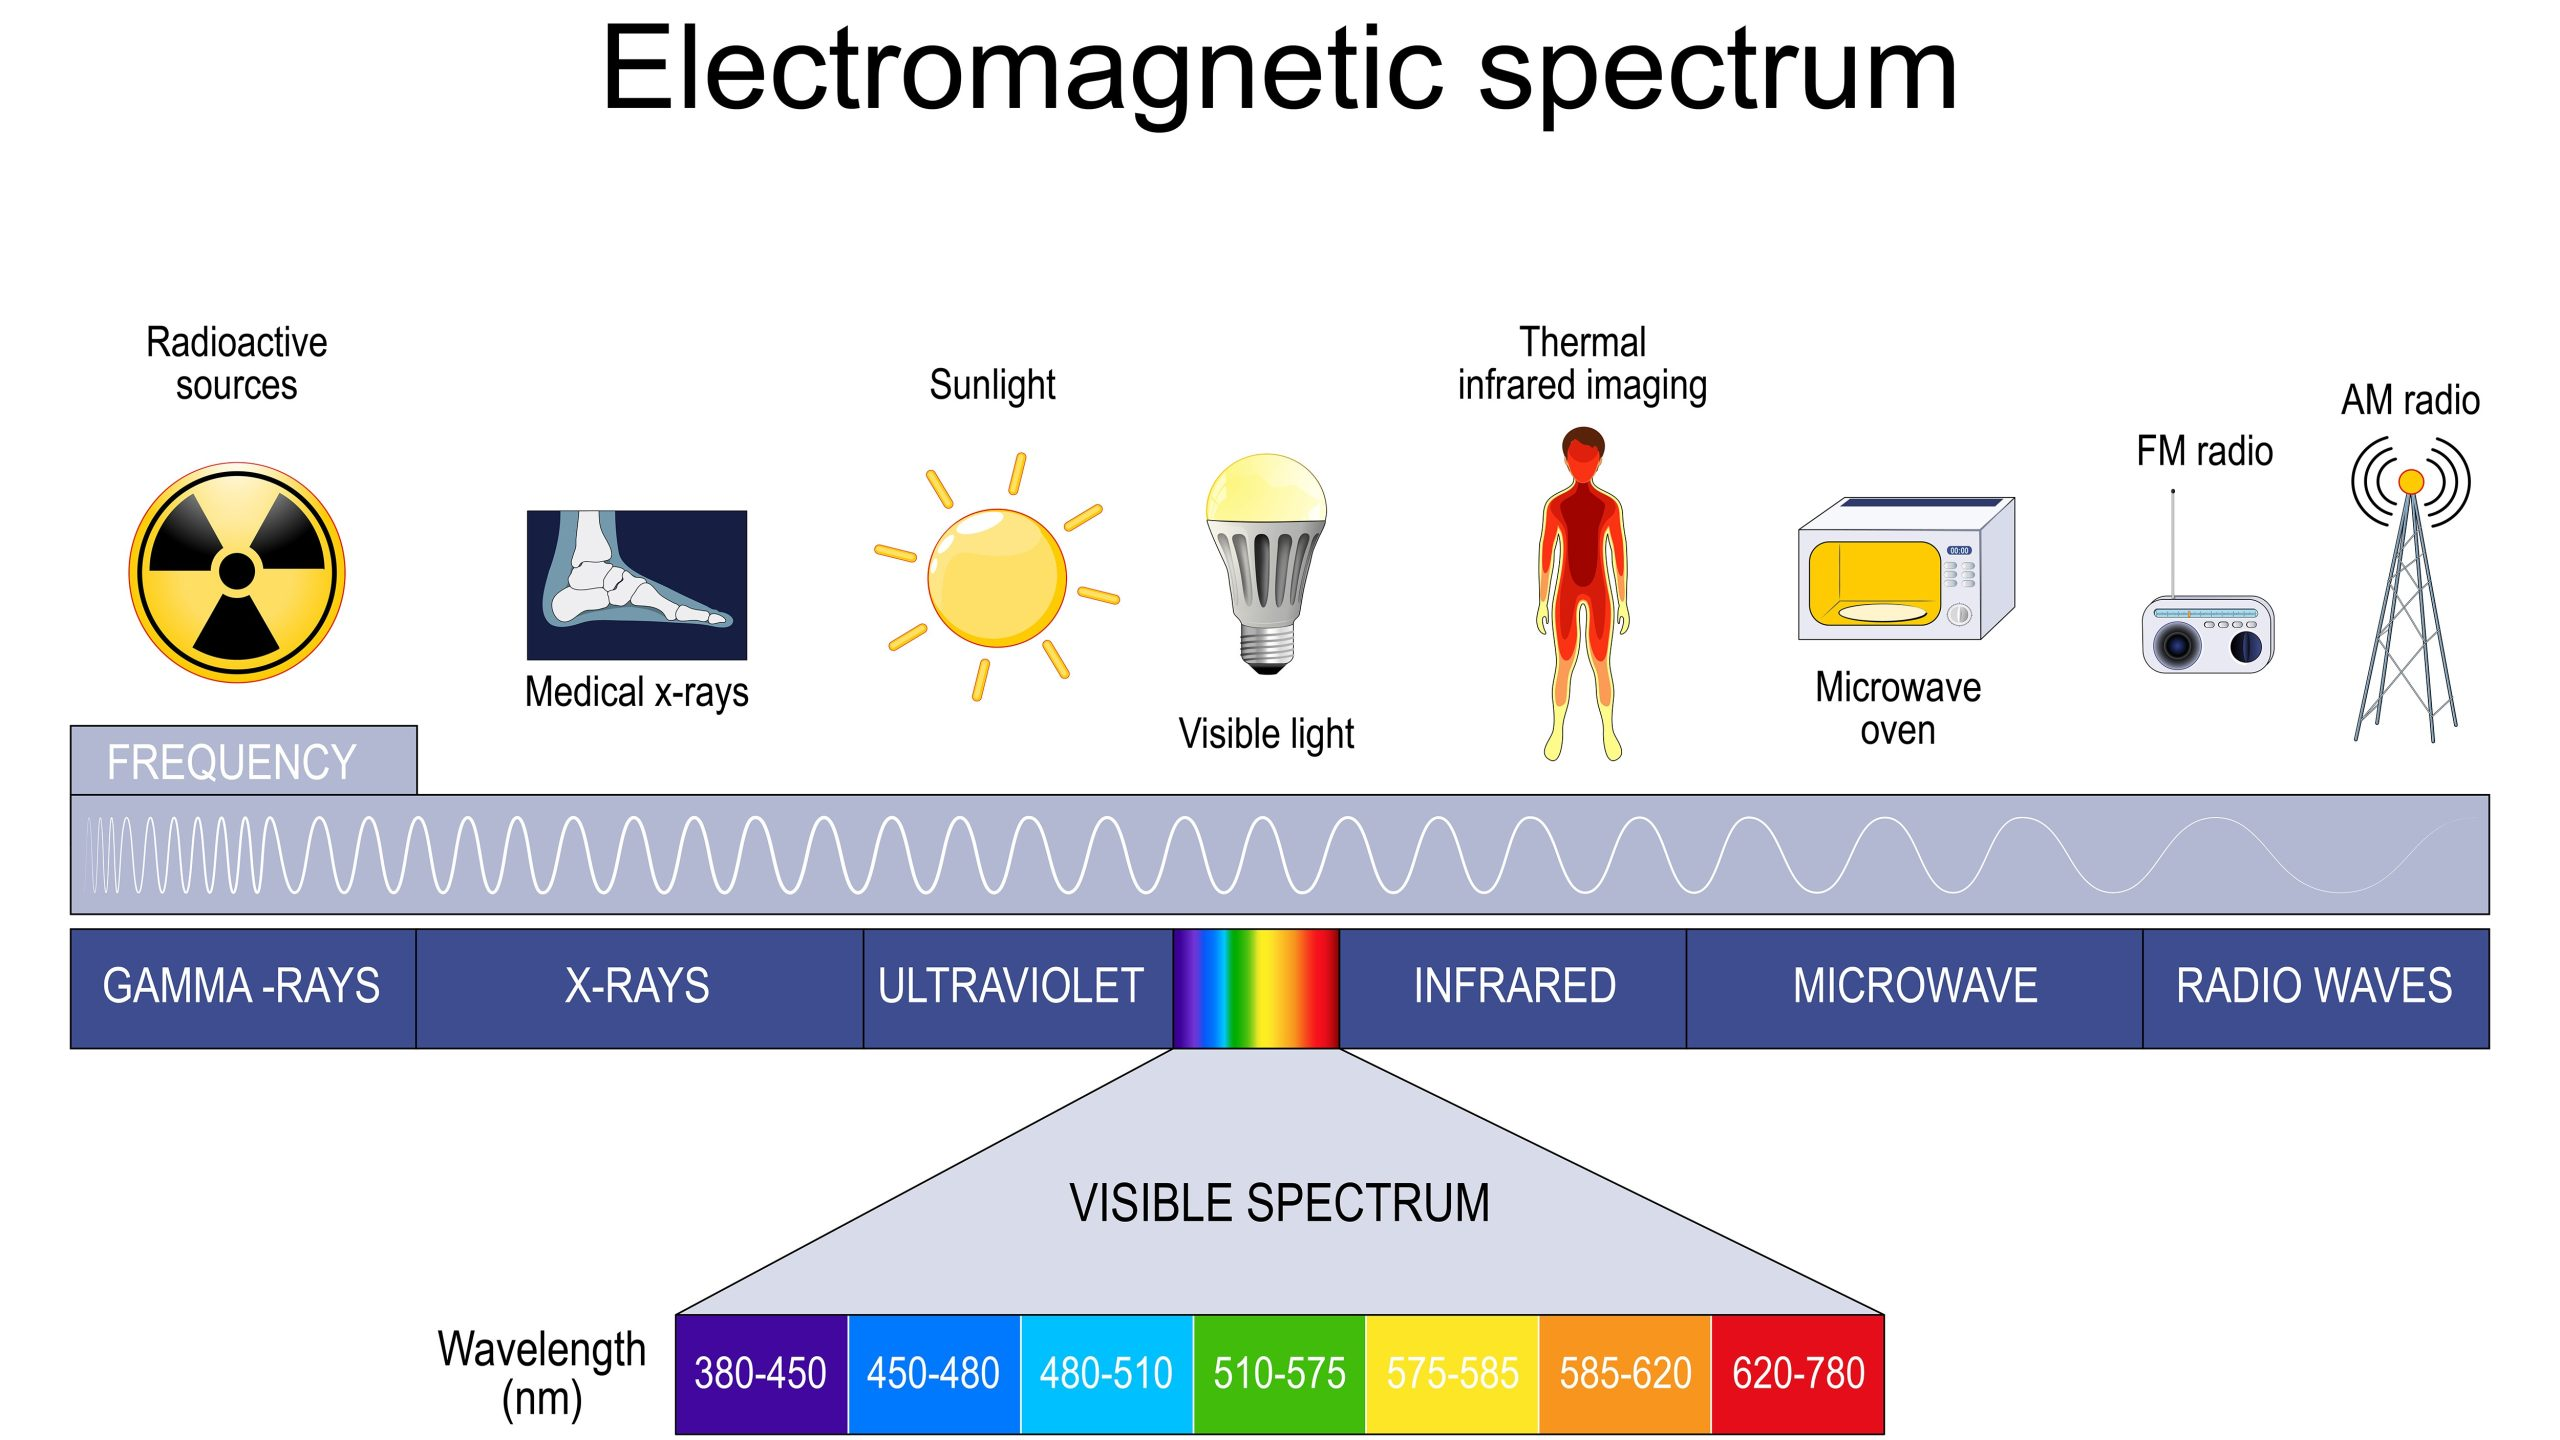
\includegraphics[width=\textwidth, height=300pt, trim={100 400 0 200},clip]{images/1490370103.jpg}

%%\caption{Eigenvalues.}
%\label{fig:pemd_0114}
 \end{figure}

%\end{minipage}
\end{textblock*}


\begin{textblock*}{1000pt}(3400pt,1000pt)
%\centering
%\rotatebox{90}{
%  \large \textbf{Have you ever seen a blue laser?}
{\huge\textbf {4. Interest}} \\\vspace{30pt}
%% \begin{minipage}{0.6\linewidth}
% \begin{figure}[tp]
% 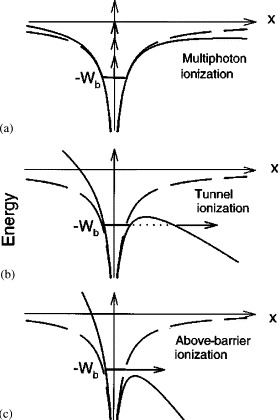
\includegraphics[scale=2., trim={0 0 0 0},clip]{images/phenomena.png} \\\vspace{100pt}
% 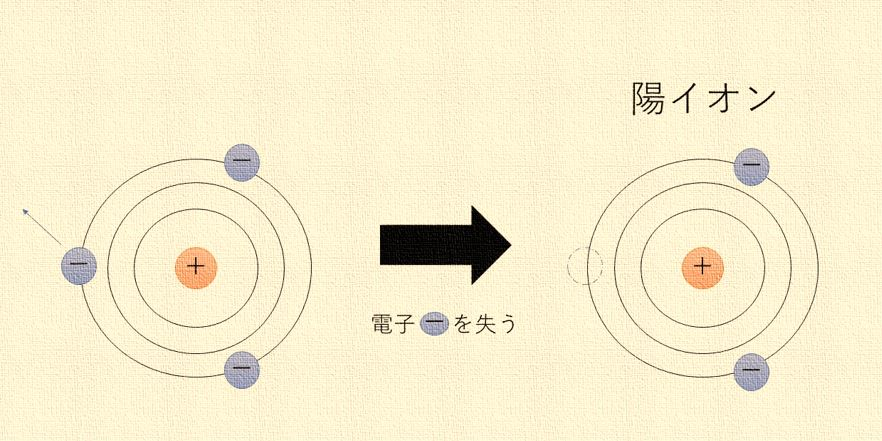
\includegraphics[scale=2., trim={0 0 0 0},clip]{images/ionization.jpg} \\
%%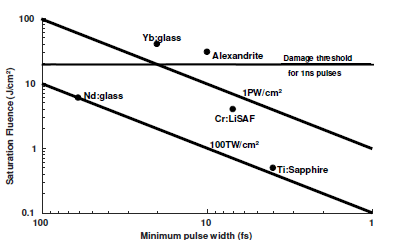
\includegraphics[scale=2., trim={0 0 0 0},clip]{images/intensity_medium.png} \\
%%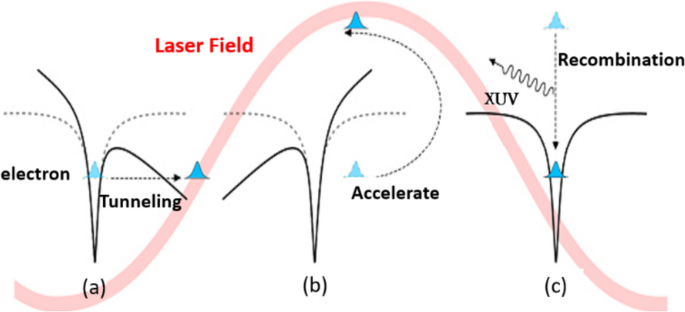
\includegraphics[scale=.50, trim={0 0 0 0},clip]{images/hhg_process.png}
%
%%%\caption{Eigenvalues.}
%%\label{fig:pemd_0114}
% \end{figure}
%
%%\end{minipage}
\begin{enumerate}
\Large
\item From different ionizations can be obtained
\begin{itemize}
\large
\item[$\bullet$] electrons with even more energy (MPI)
\item[$\bullet$] a laser more energetic than the one we used (HHG)
\item[$\bullet$] electrons ionized even with insufficient energy (TI)
\end{itemize}
\vspace{50pt}
\item Multiphoton Ionization (MPI)
\begin{itemize}
\large
\item[$\bullet$] electron is ionized by many photons instead of one
\item[$\bullet$] allows to ionize even with insufficient photon energy
\end{itemize}
\vspace{50pt}
\item High Harmonic Generation (HHG)
\begin{itemize}
\large
\item[$\bullet$] allows to multiply laser energy manyfold
\end{itemize}
\end{enumerate}
\vspace{100pt}
{\huge\textbf {5. More applications}} \\\vspace{30pt}
\begin{itemize}
\large
\item Quantum imagery technics (MRI, LIED) allowing to scan 
the body or the molecules
\item High resolution camera allowing to track the movement of atoms 
at the femtosecond scale
\item Attosecond physics in general...
\end{itemize}



\end{textblock*}


\end{frame}
\end{document}
